\documentclass[12pt,letterpaper]{article}
\usepackage[utf8]{inputenc}

% Ajustamos los márgenes para corregir las advertencias de fancyhdr
\usepackage[letterpaper, margin=1in, bottom=2.5in, top=1.2in]{geometry}

% Cargamos primero el paquete fancyhdr
\usepackage{fancyhdr}
% Corregimos los parámetros headheight y footskip
\setlength{\headheight}{15pt} % Al menos 14.49998pt según la advertencia
\setlength{\footskip}{72pt}   % Al menos 71.60547pt según la advertencia

\usepackage{xcolor}
\usepackage{amsmath}
\usepackage{anyfontsize}
\usepackage{graphicx}
\usepackage{tikz} % Necesario para los elementos gráficos
\usepackage{listings} % Para resaltado de sintaxis
\usepackage{sourcesanspro}
\renewcommand{\familydefault}{\sfdefault}
\usepackage{fontawesome5}
\usepackage{titlesec}
\usepackage{setspace}
\usepackage{hyperref}
\usepackage{mdframed} % Para marcos más estables
\usepackage{qrcode} % Paquete para generar códigos QR
\usepackage{eso-pic} % For background image

% Cargar tikz y la biblioteca de cajitas para mdframed
\usetikzlibrary{calc,shapes,positioning}

% IMPORTANT: Force the text color to be white for the entire document
\AtBeginDocument{\color{primaryColor}}

% Colors updated with better contrast
\definecolor{myblue}{cmyk}{1.0,0.8,0.05,0.20}
\definecolor{bgColor}{RGB}{15, 22, 36}  % Very dark blue, almost black background
\definecolor{primaryColor}{RGB}{255, 255, 255}  % White text - full white for better contrast
\definecolor{accentColor}{RGB}{255, 212, 59}  % Python Yellow - mismo del original
\definecolor{pythonBlue}{RGB}{120, 180, 255}  % Azul Python más claro para mejor contraste
\definecolor{secondaryColor}{RGB}{220, 230, 240}  % Lighter blue-gray for better contrast
\definecolor{terminalBg}{RGB}{22, 22, 22}  % Terminal background remains dark
\definecolor{terminalFrame}{RGB}{40, 40, 40}  % Terminal frame slightly darker
\definecolor{lineNumberColor}{RGB}{100, 100, 100}  % Color más sutil para los números de línea
\definecolor{dividerColor}{RGB}{60, 70, 90}  % Color más sutil para la línea divisoria

% Colores mejorados para el código con mayor contraste
\definecolor{codeTextColor}{RGB}{255, 255, 255}  % Blanco puro para el texto básico
\definecolor{codeKeywordColor}{RGB}{135, 206, 250}  % Azul cielo para palabras clave
\definecolor{codeCommentColor}{RGB}{144, 238, 144}  % Verde claro para comentarios
\definecolor{codeStringColor}{RGB}{255, 215, 135}  % Amarillo para strings
\definecolor{codeMethodColor}{RGB}{255, 160, 122}  % Naranja claro para métodos
\definecolor{codeFunctionColor}{RGB}{255, 215, 0}  % Dorado para funciones - como en el original
\definecolor{codeNumberColor}{RGB}{255, 255, 150}  % Amarillo claro para números

% Set page background color
\pagecolor{bgColor}

% Hyperref configuration
\hypersetup{
    colorlinks=true,
    linkcolor=accentColor,
    filecolor=accentColor,
    urlcolor=accentColor,
}

% Configuración básica para listings que evita problemas con saltos de página
\lstset{
  language=Python,
  basicstyle=\normalsize\ttfamily\bfseries\color{codeTextColor}, % Tamaño reducido, en blanco y negrita
  backgroundcolor=\color{terminalBg},
  commentstyle=\color{codeCommentColor},
  keywordstyle=\color{codeKeywordColor},
  stringstyle=\color{codeStringColor},
  numberstyle=\color{lineNumberColor}, % Números de línea más sutiles
  breaklines=true,
  breakatwhitespace=true,
  tabsize=4,
  showstringspaces=false,
  frame=none,
  xleftmargin=15pt,
  xrightmargin=0pt,
  aboveskip=10pt,
  belowskip=10pt,
  numbers=left,
  numbersep=8pt,
  extendedchars=true,
  keepspaces=true,
  columns=flexible,
  lineskip=6pt, % Espacio entre líneas ligeramente reducido
  % Keywords de Python (palabras reservadas)
  morekeywords={self, yield, lambda, with, as, from, True, False, None, import, in, for, 
                if, elif, else, while, return, def, class, try, except, finally, raise, 
                break, continue, global, nonlocal, pass, assert, del, yield from},
  % Funciones incorporadas resaltadas de manera distinta
  emph={[2]print,range,sum,int,str,float,list,dict,set,tuple,next,len,type,map,filter,
         reduce,zip,enumerate,sorted,reversed,min,max,open,any,all},
  emphstyle={[2]\color{codeFunctionColor}}
}

% TERMINAL ESTILO MAC MEJORADA CON BOTONES A LA IZQUIERDA Y MENOS ESPACIO SUPERIOR
\newenvironment{macterminal}{%
    \begin{mdframed}[
        linecolor=terminalFrame,
        backgroundcolor=terminalBg,
        roundcorner=5pt,
        skipabove=10pt,
        skipbelow=10pt,
        linewidth=1pt,
        innertopmargin=10pt, % Reducido
        frametitle={%
            \tikz[baseline=(current bounding box.east), outer sep=0pt]{
                \fill[red!80!black] (0,0) circle (5pt);
                \fill[yellow!80!black] (0.7,0) circle (5pt);
                \fill[green!70!black] (1.4,0) circle (5pt);
            }
        },
        frametitlealignment=\raggedright, % Alineado a la izquierda
        frametitleaboveskip=8pt, % Espacio entre el título y el borde superior
        frametitlebelowskip=0pt, % Reducir el espacio entre el título y el contenido
    ]
    % No necesitamos más espacio vertical aquí
}{%
    \end{mdframed}%
}

% Utilities
\newcommand{\verspace}{\vspace{10pt}}

% Section styling - Esquema más elegante y mejorado contraste
\titleformat{\section}
  {\LARGE\bfseries\color{primaryColor}} % Secciones principales en blanco para mejor contraste y más grandes
  {\thesection. }
  {0pt}
  {}
  []

\titleformat{\subsection}
  {\Large\bfseries\color{accentColor}} % Subsecciones en amarillo como original
  {\thesubsection. }
  {0pt}
  {}
  []

\titleformat{\subsubsection}
  {\large\bfseries\color{pythonBlue}} % Subsubsecciones en azul Python más claro y más grandes
  {\thesubsubsection. }
  {0pt}
  {}
  []

% Spacing for sections
\titlespacing*{\section}{0pt}{20pt}{10pt}
\titlespacing*{\subsection}{0pt}{15pt}{7pt}
\titlespacing*{\subsubsection}{0pt}{10pt}{5pt}

% Configure header and footer
\pagestyle{fancy}
\fancyhf{}

% Crear un encabezado elegante para todas las páginas (excepto la portada)
\fancyhead[L]{
    
\begin{tikzpicture}[remember picture, overlay]
        % Rectángulo de fondo para la sección Python
        \fill[pythonBlue, rounded corners=3pt] (0,0) rectangle (2.2cm,0.7cm);
        % Texto Python
        \node[text=primaryColor, font=\bfseries] at (1.1cm,0.35cm) {PYTHON};
        
        % Pequeño separador
        \fill[secondaryColor] (2.35cm,0.1cm) rectangle (2.40cm,0.6cm);
        
        % Texto para decoradores con color de acento
        \node[text=accentColor, font=\bfseries, anchor=west] at (2.35cm,0.35cm) {DECORATORS};
    \end{tikzpicture}
}

% Línea de encabezado
\renewcommand{\headrulewidth}{0pt}

% Línea divisoria más sutil
\renewcommand{\footrule}{
  \vspace{0.5cm}
  \noindent\makebox[\linewidth]{\color{dividerColor}\rule{\linewidth}{0.2pt}}
  \vspace{0.5cm}
}
\renewcommand{\footrulewidth}{0.2pt}
\renewcommand{\footruleskip}{1cm}

% Configure footer with profile info
\fancyfoot[C]{
    \vspace*{0.2cm}
    \noindent
    \begin{minipage}{\textwidth}
        \begin{flushleft}
            % Profile image placeholder with TikZ
            \raisebox{0.7cm}{
            \begin{tikzpicture}[baseline]
                \path[fill=bgColor] (0,0) circle (0.8cm);
                \clip (0,0) circle (0.8cm);
                \node at (0,0) {
                    % Placeholder for profile image
                    
\includegraphics[width=1.6cm,height=1.6cm]{../../Images/profile-image.jpeg}
                };
            \end{tikzpicture}
            }
            \begin{minipage}[b]{0.8\textwidth}
                % Name
                {\large\bfseries\color{primaryColor}Alejandro Sánchez Yalí}
                
                % Professional description
                \par\vspace{1pt}
                {\small\color{secondaryColor}Software Developer | AI \& Blockchain Enthusiast}
                
                % Contact
                \par\vspace{1pt}
                {\small\color{accentColor}\faGlobe\hspace{5pt}\color{secondaryColor}www.asanchezyali.com}
            \end{minipage}
        \end{flushleft}
        \vspace{8pt} % Space at bottom
    \end{minipage}
}

% Estilo para la portada (sin encabezado ni pie de página)
\fancypagestyle{plain}{
    \fancyhf{}
    \renewcommand{\headrulewidth}{0pt}
    \renewcommand{\footrulewidth}{0pt}
}

% Bullet styling for lists
\renewcommand{\labelitemi}{\textcolor{accentColor}{$\bullet$}} % Primer nivel de viñetas en amarillo
\renewcommand{\labelitemii}{\textcolor{pythonBlue}{$\circ$}} % Segundo nivel de viñetas en azul

% Aumentar globalmente el tamaño de texto un 20%
\usepackage{relsize}
\AtBeginDocument{\relsize{1}} % Incrementa la fuente en aproximadamente un 20%

% Comando simplificado para la etiqueta Python
\newcommand{\languagetag}[1]{
    \begin{tikzpicture}[baseline]
        \node[fill=pythonBlue, text=primaryColor, rounded corners=5pt, inner sep=7pt] {
            {\normalsize\textbf{#1}}
        };
    \end{tikzpicture}
}

% Alternativa usando una versión modificada de la URL
\newcommand{\elegantqr}[2]{
    \qrcode[height=2.5cm]{#1}
    \\[0.1cm]
    {\hspace{0.2cm}\color{primaryColor}\small #2\par}
}

% Background image setup
\newcommand{\BackgroundPic}{%
    \put(0,0){%
        \begin{tikzpicture}[remember picture, overlay]
            % Place the background image to cover the whole page
            \node[inner sep=0pt] at (current page.center) {
                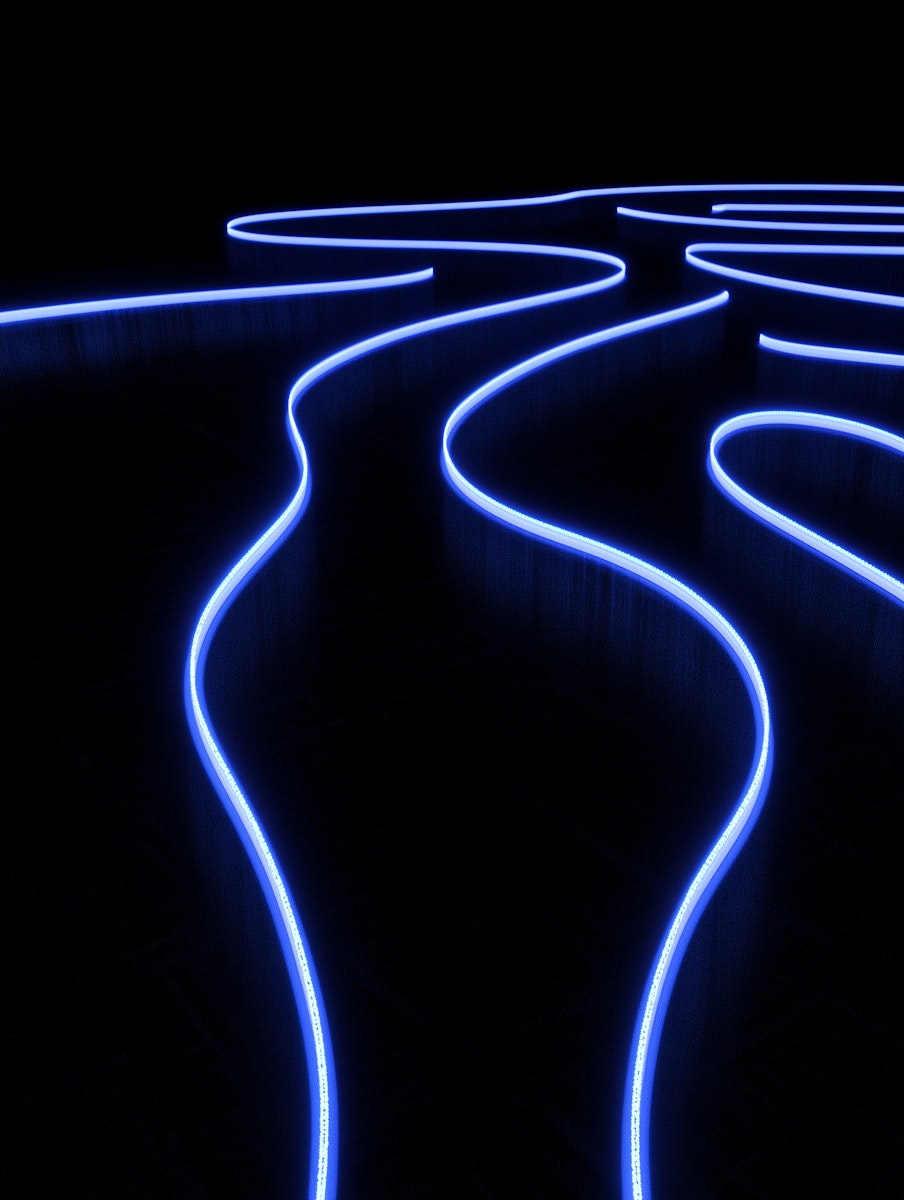
\includegraphics[width=\paperwidth,height=\paperheight]{../../Images/Glowing Neon Abstract.jpeg}
            };
            % Add a semi-transparent dark overlay
            \fill[black, opacity=0.7] (current page.south west) rectangle (current page.north east);
        \end{tikzpicture}%
    }%
}

\newcommand{\titlepagecontents}{%
    \AddToShipoutPicture*{\BackgroundPic}
    \vspace*{2cm}
    \begin{flushleft}
    \noindent\languagetag{Python}\\[0.4cm]
    \noindent{\fontsize{48}{52}\bfseries\color{primaryColor}Python \color{accentColor}Decorators\par}
    \vspace{0.3cm}
    \noindent{\fontsize{18}{52}\color{secondaryColor}Enhancing Functions with Elegant Wrappers\par}
    \vspace{0.3cm}
    \noindent{\color{secondaryColor}\today\par}
    \vspace{2cm}
    \elegantqr{https://github.com/asanchezyali/social-media-posts/tree/main/Python/Decorators}{Source Code}
    \end{flushleft}
}

\newcommand{\finalpagecontents}{%
    \AddToShipoutPicture*{\BackgroundPic}
    \vspace*{3cm}
    \begin{flushleft}
    \languagetag{Feedback}\\[0.4cm]
    {\fontsize{46}{52}\bfseries\color{primaryColor}Found this \color{accentColor}helpful?\par}
    \vspace{0.3cm}
    {\fontsize{18}{52}\color{secondaryColor}Save, comment and share\par}  
    \vspace{0.3cm}
    {\color{secondaryColor}\today\par}
    \end{flushleft}
}

\begin{document}
\color{primaryColor} % Explicitly set text color to white for the entire document
\setlength{\parindent}{0pt} % Remove paragraph indentation

\begin{titlepage}
    % Eliminamos todos los espacios adicionales para asegurar la alineación
    \titlepagecontents
\end{titlepage}

\section{Introduction to Python Decorators}

Python decorators are a powerful feature that allow developers to modify or enhance functions and classes without
changing their core implementation. In essence, decorators are a design pattern that lets you "wrap" one function with
another function to extend its behavior.

\subsection{What Are Decorators?}

At their core, decorators are a form of metaprogramming – code that manipulates other code. They provide a clean syntax to modify the behavior of functions or classes using the \textbf{\textcolor{accentColor}{@}} symbol.

\begin{itemize}
    \item \textbf{\textcolor{pythonBlue}{Higher-Order Functions:}} Functions that take another function as an argument
    \item \textbf{\textcolor{pythonBlue}{Syntactic Sugar:}} The \textbf{\textcolor{accentColor}{@decorator}} syntax is equivalent to \textbf{\textcolor{accentColor}{function = decorator(function)}}
    \item \textbf{\textcolor{pythonBlue}{Non-Invasive:}} Add functionality without modifying the original code
    \item \textbf{\textcolor{pythonBlue}{Reusability:}} Apply the same behavior across multiple functions
\end{itemize}

\section{Basic Decorator Pattern}

The fundamental decorator pattern consists of a function that takes another function as input and returns a new function with enhanced behavior:

\begin{macterminal}
\begin{lstlisting}
def my_decorator(func):
    def wrapper():
        print("Something is happening before the function is called.")
        func()
        print("Something is happening after the function is called.")
    return wrapper

@my_decorator
def say_hello():
    print("Hello!")

# Call the decorated function
say_hello()

# Output:
# Something is happening before the function is called.
# Hello!
# Something is happening after the function is called.
\end{lstlisting}
\end{macterminal}

The \textbf{\textcolor{accentColor}{@my\_decorator}} syntax is equivalent to:

\begin{macterminal}
\begin{lstlisting}
def say_hello():
    print("Hello!")

# Manually apply the decorator
say_hello = my_decorator(say_hello)
\end{lstlisting}
\end{macterminal}

\section{Decorating Functions with Arguments}

Real-world functions often have arguments. Decorators need to handle these arguments correctly:

\begin{macterminal}
\begin{lstlisting}
import functools

def decorator_with_args(func):
    @functools.wraps(func)  # Preserves the original function's metadata
    def wrapper(*args, **kwargs):
        print(f"Calling {func.__name__} with arguments: {args}, {kwargs}")
        result = func(*args, **kwargs)
        print(f"Function {func.__name__} returned: {result}")
        return result
    return wrapper

@decorator_with_args
def add(a, b):
    """Add two numbers."""
    return a + b

# Call the decorated function
result = add(3, 5)
print(f"Result: {result}")

# Output:
# Calling add with arguments: (3, 5), {}
# Function add returned: 8
# Result: 8

# Check that metadata is preserved
print(add.__name__)  # 'add' (not 'wrapper')
print(add.__doc__)   # 'Add two numbers.'
\end{lstlisting}
\end{macterminal}

\section{Decorators with Parameters}

Sometimes we need to create decorators that accept their own parameters:

\begin{macterminal}
\begin{lstlisting}
def repeat(times=2):
    """A decorator that runs a function multiple times"""
    def decorator(func):
        @functools.wraps(func)
        def wrapper(*args, **kwargs):
            result = None
            for _ in range(times):
                result = func(*args, **kwargs)
            return result
        return wrapper
    return decorator

@repeat(times=3)
def greet(name):
    print(f"Hello, {name}!")
    return name

# Call the decorated function
greet("World")

# Output:
# Hello, World!
# Hello, World!
# Hello, World!
\end{lstlisting}
\end{macterminal}

Note the triple-level nesting required for parameterized decorators:
\begin{itemize}
    \item \textbf{\textcolor{pythonBlue}{Level 1:}} \textbf{\textcolor{accentColor}{repeat()}} - handles decorator parameters
    \item \textbf{\textcolor{pythonBlue}{Level 2:}} \textbf{\textcolor{accentColor}{decorator()}} - accepts the function being decorated
    \item \textbf{\textcolor{pythonBlue}{Level 3:}} \textbf{\textcolor{accentColor}{wrapper()}} - handles the function's arguments
\end{itemize}

\section{Practical Applications}

Decorators shine in many real-world scenarios where they help separate cross-cutting concerns from business logic.

\subsection{Timing Functions}

Measuring execution time without cluttering your functions:

\begin{macterminal}
\begin{lstlisting}
import time
import functools

def timing_decorator(func):
    @functools.wraps(func)
    def wrapper(*args, **kwargs):
        start_time = time.time()
        result = func(*args, **kwargs)
        end_time = time.time()
        print(f"{func.__name__} ran in {end_time - start_time:.4f} seconds")
        return result
    return wrapper

@timing_decorator
def slow_function():
    time.sleep(1)
    return "Function complete"

slow_function()
# Output: slow_function ran in 1.0009 seconds
\end{lstlisting}
\end{macterminal}

\subsection{Caching Results}

Improve performance by storing previously calculated results:

\begin{macterminal}
\begin{lstlisting}
def memoize(func):
    """Cache the return value of function calls"""
    cache = {}
    
    @functools.wraps(func)
    def wrapper(*args):
        if args not in cache:
            cache[args] = func(*args)
        return cache[args]
    return wrapper

@memoize
def fibonacci(n):
    """Calculate the nth Fibonacci number recursively"""
    if n <= 1:
        return n
    return fibonacci(n-1) + fibonacci(n-2)

# Without memoization, this would be extremely slow
print(fibonacci(35))  # Fast calculation using cached values
\end{lstlisting}
\end{macterminal}

\subsection{Authentication and Authorization}

Control access to functions based on user roles:

\begin{macterminal}
\begin{lstlisting}
def requires_auth(role="user"):
    def decorator(func):
        @functools.wraps(func)
        def wrapper(user, *args, **kwargs):
            # Check if user has required role
            if not hasattr(user, "role") or user.role != role:
                raise PermissionError(f"User must have '{role}' role")
            return func(user, *args, **kwargs)
        return wrapper
    return decorator

class User:
    def __init__(self, name, role):
        self.name = name
        self.role = role

@requires_auth(role="admin")
def delete_item(user, item_id):
    print(f"User {user.name} deleted item {item_id}")

# Admin user can delete items
admin = User("Alice", "admin")
delete_item(admin, 42)

# Regular user will get an error
regular_user = User("Bob", "user")
try:
    delete_item(regular_user, 42)
except PermissionError as e:
    print(e)  # Output: User must have 'admin' role
\end{lstlisting}
\end{macterminal}

\subsection{Validation and Type Checking}

Ensure function inputs meet requirements:

\begin{macterminal}
\begin{lstlisting}
def validate_types(**param_types):
    def decorator(func):
        @functools.wraps(func)
        def wrapper(*args, **kwargs):
            # Get function parameter names
            import inspect
            sig = inspect.signature(func)
            bound_args = sig.bind(*args, **kwargs)
            
            # Check each parameter type
            for param_name, param_type in param_types.items():
                if param_name in bound_args.arguments:
                    value = bound_args.arguments[param_name]
                    if not isinstance(value, param_type):
                        raise TypeError(
                            f"Parameter '{param_name}' must be {param_type.__name__}"
                        )
            return func(*args, **kwargs)
        return wrapper
    return decorator

@validate_types(name=str, age=int)
def create_user(name, age):
    return f"User {name}, age {age} created"

print(create_user("Alice", 30))  # Works
try:
    print(create_user("Bob", "thirty"))  # TypeError
except TypeError as e:
    print(e)  # Output: Parameter 'age' must be int
\end{lstlisting}
\end{macterminal}

\section{Built-in Decorators}

Python includes several built-in decorators that demonstrate the power of this pattern.

\subsection{Property Decorator}

The \textbf{\textcolor{accentColor}{@property}} decorator transforms methods into attribute-like accessors:

\begin{macterminal}
\begin{lstlisting}
class Temperature:
    def __init__(self, celsius=0):
        self._celsius = celsius
        
    @property
    def celsius(self):
        """Get the current temperature in Celsius."""
        return self._celsius
        
    @celsius.setter
    def celsius(self, value):
        if value < -273.15:
            raise ValueError("Temperature below absolute zero!")
        self._celsius = value
        
    @property
    def fahrenheit(self):
        """Get the current temperature in Fahrenheit."""
        return self._celsius * 9/5 + 32
        
    @fahrenheit.setter
    def fahrenheit(self, value):
        self.celsius = (value - 32) * 5/9

# Using the properties
temp = Temperature()
temp.celsius = 25
print(f"{temp.celsius} C is {temp.fahrenheit} F")

# Setting in Fahrenheit automatically updates Celsius
temp.fahrenheit = 68
print(f"{temp.fahrenheit} F is {temp.celsius} C")
\end{lstlisting}
\end{macterminal}

\subsection{Class and Static Method Decorators}

\begin{macterminal}
\begin{lstlisting}
class MathUtils:
    multiplier = 2
    
    def __init__(self, value):
        self.value = value
    
    def multiply(self):
        """Instance method: uses self"""
        return self.value * self.multiplier
    
    @classmethod
    def set_multiplier(cls, new_value):
        """Class method: uses cls instead of self"""
        cls.multiplier = new_value
        return cls.multiplier
    
    @staticmethod
    def is_even(num):
        """Static method: uses neither self nor cls"""
        return num % 2 == 0

# Using the different method types
math = MathUtils(5)
print(math.multiply())  # 10 (5 * 2)

# Class method affects all instances
MathUtils.set_multiplier(3)
print(math.multiply())  # 15 (5 * 3)

# Static method is independent
print(MathUtils.is_even(4))  # True
\end{lstlisting}
\end{macterminal}

\section{Decorators in the Wild}

Decorators are widely used in popular Python frameworks and libraries.

\subsection{Flask Web Framework}

Flask uses decorators for route definitions:

\begin{macterminal}
\begin{lstlisting}
from flask import Flask, request

app = Flask(__name__)

@app.route('/hello/<name>')
def hello(name):
    return f"Hello, {name}!"

@app.route('/login', methods=['POST'])
def login():
    username = request.form['username']
    password = request.form['password']
    # Authentication logic here
    return f"Welcome back, {username}!"
\end{lstlisting}
\end{macterminal}

\subsection{Django Framework}

Django uses decorators for views and authentication:

\begin{macterminal}
\begin{lstlisting}
from django.shortcuts import render
from django.contrib.auth.decorators import login_required
from django.views.decorators.http import require_POST

@login_required
def profile(request):
    # Only accessible to logged-in users
    return render(request, 'profile.html')

@require_POST
def update_profile(request):
    # Only accepts POST requests
    # Update profile logic
    return render(request, 'profile_updated.html')
\end{lstlisting}
\end{macterminal}

\section{Best Practices}

Follow these guidelines to create effective and maintainable decorators:

\begin{itemize}
    \item \textbf{\textcolor{pythonBlue}{Use functools.wraps:}} Always preserve the original function's metadata
    \item \textbf{\textcolor{pythonBlue}{Handle all arguments:}} Use \textbf{\textcolor{accentColor}{*args, **kwargs}} to support any function signature
    \item \textbf{\textcolor{pythonBlue}{Keep decorators focused:}} Each decorator should do one thing well
    \item \textbf{\textcolor{pythonBlue}{Document decorators:}} Clearly explain what your decorator does
    \item \textbf{\textcolor{pythonBlue}{Consider performance:}} Decorators add overhead to function calls
    \item \textbf{\textcolor{pythonBlue}{Test decorated functions:}} Ensure decorators don't change expected behavior
\end{itemize}

\section{Conclusion}

Python decorators embody elegant metaprogramming by providing a clean syntax for extending function and class behavior. They allow developers to apply consistent patterns across their codebase, separate concerns, and write more maintainable software.

By mastering decorators, you can:
\begin{itemize}
    \item Add cross-cutting functionality without cluttering core business logic
    \item Create reusable code patterns that can be applied consistently
    \item Solve common programming challenges with clean, readable solutions
    \item Better understand Python's powerful metaprogramming capabilities
\end{itemize}

Decorators shine brightest when they handle aspects like logging, timing, caching, authentication, and validation—allowing your core code to focus solely on its primary responsibility.

\clearpage
\thispagestyle{empty}
\finalpagecontents

\end{document}